%%%%%%%%%%%%%%%%%%%%%%
%%%%%%%%%%%%%%%%%%%%%%
%%Options for presentations (in-class) and handouts (e.g. print). 
\documentclass[pdf
,handout
]{beamer}
\usepackage{pgfpages}
\pgfpagesuselayout{2 on 1}[letterpaper,border shrink=5mm]

\graphicspath{{../}}
%%%%%%%%%%%%%%%%%%%%%%
%% Change this for different slides so it appears in bar
\usepackage{authoraftertitle}
\date{Linear Transformations: Properties}

%%%%%%%%%%%%%%%%%%%%%%
%% Upload common style file
\usepackage{../LyryxLinearAlgebraSlidesStyle}

\begin{document}
	
	%%%%%%%%%%%%%%%%%%%%%%%
	%% Title Page and Copyright Common to All Slides
	
	%Title Page
	\input ../frontmatter/titlepage.tex
	
	%LOTS Page
	%\input frontmatter/lyryxopentexts.tex
	
	%Copyright Page
	\input ../frontmatter/copyright.tex
	
	%%%%%%%%%%%%%%%%%%%%%%%%%


\section{Properties} 

%-------------- start slide -------------------------------%
\frame{\frametitle{Recall: Linear Transformations}
\begin{definition}
\pause
A transformation $T:\RR^n\rightarrow \RR^m$ is a
\alert{linear transformation} if it satisfies the following
two properties for all $\vect{x},\vect{y}\in\RR^n$ and all (scalars) $a\in\RR$.
\pause
\begin{enumerate}
\item $T(\vect{x}+\vect{y})=T(\vect{x})+T(\vect{y})$ \hfill\alert{(preservation of addition)}
\pause
\item $T(a\vect{x})=aT(\vect{x})$
\hfill\alert{(preservation of scalar multiplication)}
\end{enumerate}
\end{definition}
}
%-------------- end slide -------------------------------%



\section{Composition of Linear Transformations}
%-------------- start slide -------------------------------%
\frame{\frametitle{Composition of Linear Transformations}
\begin{definition}
Suppose $T:\RR^k\rightarrow \RR^n$ and
$S:\RR^n\rightarrow \RR^m$ are linear transformations.
\pause
The \alert{composite} (or composition) of $S$ and $T$ is
\[ S\circ T: \RR^k\rightarrow \RR^m,\]
\pause
is defined by
\[ (S\circ T)(\vect{x})=S(T(\vect{x}))  \mbox{ for all }\vect{x}\in\RR^k.\]
\pause
\begin{picture}(2,1)
\put(0.8,0.2){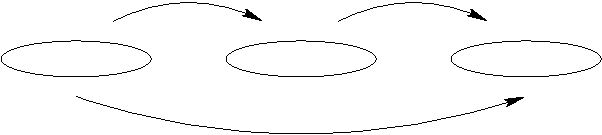
\includegraphics[scale=.75]{figures/composition.pdf}}
\put(1.08,0.53){$\RR^k$}
\put(2.22,0.53){$\RR^n$}
\put(3.36,0.53){$\RR^m$}
\put(1.67,0.7){$T$}
\put(2.81,0.7){$S$}
\put(2.13,0.26){$S\circ T$}
\end{picture}
\pause

\alert{Be careful with the order of the transformations!}
We write $S\circ T$, but it is the transformation $T$ that
is applied first, followed by the transformation $S$.
\end{definition}
}
%------------------------end slide-------------------------%

%-------------- start slide -------------------------------%
\frame{
%\begin{definition}[Equality of Transformations]
%Suppose $S:\RR^n\rightarrow\RR^m$
%and $T:\RR^n\rightarrow\RR^m$
%are transformations.
%Then $S=T$ if and only if $S(\vect{x})=T(\vect{x})$ for every $\vect{x}\in\RR^n$.
%\end{definition}
%\pause
\begin{theorem}\em
Let $\RR^k\stackrel{T}{\rightarrow}
\RR^n\stackrel{S}{\rightarrow} \RR^m$
be linear transformations,
and suppose that $S$ is induced by matrix $A$, 
and $T$ is induced by matrix $B$.
Then $S\circ T$ is a linear transformation, 
and $S\circ T$ is induced by the matrix $AB$.
\end{theorem}
\pause
\begin{example}
Let $S:\RR^2\to\RR^2$ and $T:\RR^2\to\RR^2$ be linear
transformations defined by
\[ S\left[\begin{array}{c} x \\ y \end{array}\right]
= \left[\begin{array}{c} x \\ -y \end{array}\right]
\mbox{ and }
T\left[\begin{array}{c} x \\ y \end{array}\right]
= \left[\begin{array}{c} -y \\ x \end{array}\right]
\mbox{ for all }
\left[\begin{array}{c} x \\ y \end{array}\right]
\in\RR^2.  \]

\end{example}
}
%------------------------end slide-------------------------%

%-------------- start slide -------------------------------%
\frame{
\begin{example}[continued]
Then $S$ and $T$ are induced by matrices
\[ A=\left[\begin{array}{rr} 1 & 0 \\ 0 & -1 \end{array}\right]
\mbox{ and }
B=\left[\begin{array}{rr} 0 & -1 \\ 1 & 0 \end{array}\right],
\]
respectively.
\pause
The composite of $S$ and $T$ is the transformation
$S\circ T:\RR^2\to\RR^2$ 
\pause
defined by 
\[ (S\circ T)\left[\begin{array}{c} x \\ y \end{array}\right]
= S\left( T\left[\begin{array}{c} x \\ y \end{array}\right]\right),\]
\pause
and has matrix (or is induced by the matrix)
\[ AB =\left[\begin{array}{rr} 0 & -1 \\ -1 & 0 \end{array}\right].\]
\end{example}
}
%------------------------end slide-------------------------%

%-------------- start slide -------------------------------%
\frame{
\begin{example}[continued]
Therefore the composite of $S$ and $T$ is the linear transformation
\[ (S\circ T)\left[\begin{array}{c} x \\ y \end{array}\right]
=AB\left[\begin{array}{c} x \\ y \end{array}\right]
=\left[\begin{array}{rr} 0 & -1 \\ -1 & 0 \end{array}\right]
\left[\begin{array}{c} x \\ y \end{array}\right]
=\left[\begin{array}{c} -y \\ -x \end{array}\right],
\]
for each $\left[\begin{array}{c} x \\ y \end{array}\right]\in\RR^2$.
\pause
\bigskip

Compare this with the composite of $T$ and $S$ which is the linear
transformation
\[ (T\circ S)\left[\begin{array}{c} x \\ y \end{array}\right]
=\left[\begin{array}{c} y \\ x \end{array}\right],
\]
for each $\left[\begin{array}{c} x \\ y \end{array}\right]\in\RR^2$.

\end{example}
}
%------------------------end slide-------------------------%

\section{Inverse of a Linear Transformations}
%-------------- start slide -------------------------------%
\frame{\frametitle{Inverse of a Linear Transformations}
\begin{definition}
\pause
Suppose $T:\RR^n\rightarrow\RR^n$ and
$S:\RR^n\rightarrow\RR^n$ are 
linear transformations such that
for each $\vect{x}\in\RR^n$,
\pause
\vspace*{-.25in}

\[ (S\circ T)(\vect{x}) = \vect{x} \mbox{ and }
(T\circ S)(\vect{x}) = \vect{x} .\]
\vspace*{-.22in}

\pause
Then $T$ and $S$ are \alert{invertible} transformations;
\pause
$S$ is called \alert{an inverse of $T$},
\pause
and $T$ is called \alert{an inverse of $S$}.
\textcolor{blue}{(Geometrically, $S$ reverses the action of $T$,
and $T$ reverses the action of $S$.)}
\end{definition}
\pause
\pause
\begin{theorem}\em
Let $T:\RR^n\rightarrow \RR^n$ be a matrix transformation induced
by matrix $A$.
Then $A$ is invertible if and only if $T$ has an
inverse.
In the case where $T$ has an inverse, the inverse is unique and
is denoted $T^{-1}$.
Furthermore, $T^{-1}:\RR^n\rightarrow \RR^n$ is induced
by the matrix $A^{-1}$.
\end{theorem}
}
%------------------------end slide-------------------------%

%-----------------------start slide-----------------------%
\frame{\frametitle{Inverse of a Linear Transformations}
\begin{block}
{Fundamental Identities relating $T$ and $T^{-1}$}
\begin{enumerate}
\item
$T^{-1}\circ T = 1_{\RR^n}$
\item
$T\circ T^{-1} = 1_{\RR^n}$
\end{enumerate}
\end{block}
}
%---------------------end slide----------------------------%

%-------------- start slide -------------------------------%
\frame{
\begin{example}
Let $T : \mathbb{R}^2 \mapsto \mathbb{R}^2$ be a transformation given by 
\[
T \left[ 
\begin{array}{r}
x \\
y
\end{array}\right]
 = 
\left[
\begin{array}{c}
x + y \\
y
\end{array}
\right]
\]

Then $T$ is a linear transformation induced by $A = \left[ \begin{array}{rr}
1 & 1 \\
0 & 1 
\end{array} \right]$. 

\pause 

Notice that the matrix $A$ is invertible. Therefore the transformation $T$ has an inverse, $T^{-1}$, induced by
\[
A^{-1} = \left[ 
\begin{array}{rr}
1 & -1 \\
0 & 1
\end{array} \right]
\]
 

\end{example}
}
%------------------------end slide-------------------------%

%------------------------ start slide-------------------%
\frame{
\begin{example}[continued]
Consider the action of $T$ and $T^{-1}$.

\pause

\[
T \left[ \begin{array}{r}
x \\
y
\end{array} \right] = \left[ \begin{array}{rr}
1 & 1 \\
0 & 1 
\end{array} \right] \left[ \begin{array}{r}
x \\
y
\end{array} \right]  = \left[ \begin{array}{c}
x + y \\ 
y 
\end{array} \right]
\]

\pause

\[
T^{-1} \left[ \begin{array}{c}
x + y \\
y
\end{array}\right] = \left[ \begin{array}{rr}
1 & -1 \\
0 & 1 
\end{array} \right] \left[ \begin{array}{c}
x + y \\
y
\end{array} \right] = \left[ \begin{array}{c}
x \\
y
\end{array} \right]
\]

\pause

Therefore 
\[
T^{-1} \left( T \left[ \begin{array}{c}
x \\
y
\end{array} \right] \right) = \left[ \begin{array}{c}
x \\
y
\end{array}
\right]
\]
\end{example}

}
%---------------------end slide-----------------------%




\end{document}
